\documentclass[fsharpNotes.tex]{subfiles}
\graphicspath{ {./figures/} }

\begin{document}

\chapter{Organising Code in Libraries and Application Programs}
\label{chap:modules}
\abstract{
  Introductory text about the objectivs of this chapter
  \begin{itemize}
  \item \dots
  \end{itemize}
}

In this chapter, we will focus on a number of ways to make the code available as \idx{library} functions in F\#. A library is a collection of types, values, and functions that an application program can use. A library does not perform calculations on its own.

F\# includes several programming structures to organize code in libraries: Modules, namespaces, and classes. In this chapter, we will describe modules and namespaces. Classes will be described in detail in \Cref{chap:oop}.

\section{Dotnet projects: Libraries and applications}
\label{chap:projects}
As our programs grow in size, it can be convenient to split the program over several files, e.g., by separating functionality into something which general and specific in  nature with respect the problem being solved. Examples of this is the \lstinline{List} module which contains general functions on lists, and which you have used in your programs. In this chapter, we will write our own modules, also known as libraries, and the programs using these libraries, we will call applications. Using the \lstinline[language=console]{dotnet} command-line tool, we are able to create project files which have a \lstinline[language=console]{.fsproj} suffix, which include information about which source code and packages belongs together. The \lstinline[language=console]{dotnet} command-line tool further helps structure the files on the filesystem by use of directories. As an example
\begin{codeNOutput}[label=dotnetNew,
  top=-5pt,
  bottom=-5pt,
  left=-2pt,
  right=-2pt,
]{: Creating an initial library-application file setup.}
  \begin{lstlisting}[language=console,escapechar=§]
$ dotnet new console -lang "F#" -o app
$ dotnet new classlib -lang "F#" -o library
$ dotnet add app/app.fsproj reference library/library.fsproj
$ dotnet add app/app.fsproj package "DIKU.Canvas" --version 1.0.1
\end{lstlisting}
\end{codeNOutput}
creates the files and directories shown in \Cref{fig:dotnetNewFileSystem}.
\begin{figure} % make sure figure is printed after the countRecursive
  \centering
  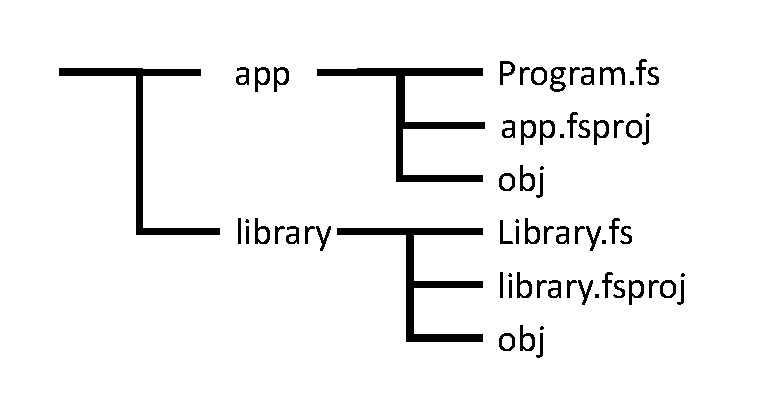
\includegraphics[width=0.5\linewidth]{dotnetNew}
  \caption{Typical initial files and directories for a library and application multifile setup and as created by \lstinline[language=console]{dotnet new} and  \lstinline[language=console]{dotnet add}.}
  \label{fig:dotnetNewFileSystem}
\end{figure}
The directories \lstinline[language=console]{obj} contains additional libraries etc.\ which dotnet needs to build projects, and can safely be ignored for now. The \lstinline[language=console]{Program.fs} and \lstinline[language=console]{Library.fs} are the default filenames for the application and the library, and the \lstinline[language=console]{.fsproj} are XML-files which describes how dotnet should combine the library and the application files etc. In this case, the \lstinline[language=console]{app.fsproj} contains
\begin{codeNOutput}[label=appFsproj,
  top=-5pt,
  bottom=-5pt,
  left=-2pt,
  right=-2pt,
]{: The initial content of \texttt{app.fsproj}.}
  \begin{lstlisting}[language=console,escapechar=§]
<Project Sdk="Microsoft.NET.Sdk">
 <PropertyGroup>
  <OutputType>Exe</OutputType>
  <TargetFramework>net6.0</TargetFramework>
 </PropertyGroup>
 <ItemGroup>
  <Compile Include="Program.fs" />
 </ItemGroup>
 <ItemGroup>
  <ProjectReference Include="..\library\library.fsproj" />
 </ItemGroup>
 <ItemGroup>
  <PackageReference Include="DIKU.Canvas" Version="1.0.1" />
 </ItemGroup>
</Project>
\end{lstlisting}
\end{codeNOutput}
which we see includes references to \lstinline[language=console]{Program.fs}, \lstinline[language=console]{library.fsproj}, and \lstinline[language=console]{DIKU.Canvas}.
Likewise, the \lstinline[language=console]{library.fsproj} file
\begin{codeNOutput}[label=libraryFsproj,
  top=-5pt,
  bottom=-5pt,
  left=-2pt,
  right=-2pt,
]{: The initial content of \texttt{library.fsproj}.}
  \begin{lstlisting}[language=console,escapechar=§]
<Project Sdk="Microsoft.NET.Sdk">
 <PropertyGroup>
  <TargetFramework>net6.0</TargetFramework>
  <GenerateDocumentationFile>true</GenerateDocumentationFile>
 </PropertyGroup>
 <ItemGroup>
  <Compile Include="Library.fs" />
 </ItemGroup>
</Project>
\end{lstlisting}
\end{codeNOutput}
contains a reference to \lstinline[language=console]{Library.fs}.

These files can be edited in any text-editor, e.g., if we wish our application source file to be called \lstinline[language=console]{Program.fsx}, we rename \lstinline[language=console]{Program.fs} to \lstinline[language=console]{Program.fsx}, in the \lstinline[language=console]{app}-directory, edit \lstinline[language=console]{app.fsproj} by replacing \lstinline[language=console]{Program.fs} with \lstinline[language=console]{Program.fsx}.

As an example, change \lstinline[language=console]{Program.fs} to become what is shown in \Cref{program},
\fsImplementation{solution/app/Program}{program}{A simple application program.}{}
change \lstinline[language=console]{Library.fs} to become what is shown in \Cref{library}, 
\fsImplementation{solution/library/Library}{library}{A simple library.}{}
and run it in \idx{compile mode} by changing to the \lstinline[language=console]{app} directory and using the \lstinline[language=console]{dotnet run} command as demonstrated in \Cref{dotnetRun}.
\begin{codeNOutput}[label=dotnetRun,
  top=-5pt,
  bottom=-5pt,
  left=-2pt,
  right=-2pt,
]{: Running an application setup with one or more project files.}
  \begin{lstlisting}[language=console,escapechar=§]
$ cd solution/app
$ dotnet run
"Greetings Jon"
\end{lstlisting}%$
\end{codeNOutput}
Assuming that \lstinline[language=console]{Program.fs} was rename to \lstinline[language=console]{Program.fsx} and \lstinline[language=console]{app.fsproj} was edited appropriately, \lstinline[language=console]{dotnet run} is almost the same as
\begin{codeNOutput}[label=dotnetRun,
  top=-5pt,
  bottom=-5pt,
  left=-2pt,
  right=-2pt,
]{: Running an application setup with one or more project files.}
  \begin{lstlisting}[language=console,escapechar=§]
$ dotnet fsi ../library/Library.fs Program.fsx
"Greetings Jon"
\end{lstlisting}%$
\end{codeNOutput}
However, \lstinline[language=console]{dotnet fsi} \idx{interprets} the library and application into executable code everytime it is called, while \lstinline[language=console]{dotnet run} only \idx{compiles} the program once. On my laptop, the time these different steps take depends on what else is running on the computer, but typical timings are
\begin{center}
  \rowcolors{2}{oddRowColor}{evenRowColor}
  \begin{tabular}{|l|l|}
    \hline
    \rowcolor{headerRowColor} Command & Time\\
    \hline
    \lstinline[language=console]|dotnet fsi ../library/Library.fs Program.fsx| & 1.2s\\
    \lstinline[language=console]|dotnet run| (first time) & 4.0s\\
    \lstinline[language=console]|dotnet run| & 1.0s\\
    \hline
\end{tabular}
\end{center}
The example application, we are studying here, is tiny, but even in this case, the repeated translation by \lstinline[language=console]{dotnet fsi} is a 16\% overhead when compared to an already compiled program, and you should expect this overhead to be larger for larger programs. However, the these tiny programs the cost of the initial compilation is 400\% and not worth the effort from a time perspective.

\section{Libraries and applications}
\label{sec:modules}
A library in F\# is expressed as a \idx{module}, which is a programming structure used to organize type declarations, values, functions, etc. The libraries should have the  suffix \lstinline[language=console]{.fs}, and here will will call them \idx{implementation files} in contrast to the signature files to be discussed below, which we will call \idx{interface files}.

A module is typically a file where the module name is declared in the first liness using the \idx[module@\lstinline{module}]{\keyword{module}} with the following syntax,
%
\begin{verbatimwrite}{\ebnf/outerModule.ebnf}
module <*ident*>
<*script*>
\end{verbatimwrite}
\syntax{\ebnf/outerModule.ebnf}{Outer module.}
%
Here, the identifier \lstinline[language=syntax]{<*ident*>} is a name not necessarily related to the filename, and the script \lstinline[language=syntax]{<*script*>} is an expression.

Consider the example from \Cref{solveQuadraticEquation} in which functions are defined for solving the values of $x$ where $f(x)=0$ for a quadratic equation. In the following, we will split this into a library of functions and an application program. For this we setup a project system of files as described in \Cref{chap:projects}, where \lstinline[language=console]{Program.fs} has been replaced by \lstinline[language=console]{Program.fsx} and the \lstinline[language=console]{app.fsproj} has been edited appropriately. The content of  \lstinline[language=console]{Library.fs} has been changed to become what is shown in \Cref{quadraticModule}, 
\fsImplementation{solve/library/Library}{quadraticModule}{A library for solving quadratic equations.}{}
and \lstinline[language=console]{Program.fsx} has been changed to what is shown in \Cref{quadraticApp}.
\fsCode{solve/app/Program}{quadraticApp}{An application using the \lstinline!Solve! module.}{}

Module files can be accompanied by \idx[signature file]{signature files} which have the suffix \lstinline[language=console]{.fsi}. A signature file contains no implementation, only type definitions. Signature files offer three distinct features:
\begin{enumerate}
\item Signature files can be used as part of the documentation of code, since type information is of paramount importance for an application programmer to use a library. 
\item Signature files may be written before the implementation file. This allows for a higher-level programming design that focuses on \emph{which} functions should be included and \emph{how} they can be composed.
\item Signature files allow for access control. Most importantly, if a type definition is not available in the signature file, then it is not available to the application program. Such definitions are private and can only be used internally in the library code. More fine-grained control related to classes is available and will be discussed in \Cref{chap:oop}.
\end{enumerate}
These features help the programmer structure the process of programming and protects the user of a library from irrelevant data and functions. A signature file contains the type definitions and the types of the values and functions the is to be exposed to the user of the library. For example, for the library in \Cref{quadraticModule}, we can define a signature files which makes the \lstinline{solveQuadraticEquation} function but not the \lstinline{discriminant} function available to the user of the library as demonstrated in \Cref{librarySignature}.
\fsSignature{solve/library/Library}{librarySignature}{A signature file for \Cref{quadraticModule}.}{}
To compile the application using the signature file, we must add the created file, e.g., \lstinline[language=console]{Library.fsi}, to \lstinline[language=console]{<Compile Include="Library.fs" />} to \lstinline[language=console]{library.fsproj} as follows
\begin{codeNOutput}[label=libraryFsprojFSI,
  top=-5pt,
  bottom=-5pt,
  left=-2pt,
  right=-2pt,
]{: The \texttt{library.fsproj} with an interface file added.}
  \begin{lstlisting}[language=console,escapechar=§]
<Project Sdk="Microsoft.NET.Sdk">
 <PropertyGroup>
  <TargetFramework>net6.0</TargetFramework>
  <GenerateDocumentationFile>true</GenerateDocumentationFile>
 </PropertyGroup>
 <ItemGroup>
  <Compile Include="Library.fsi" />
  <Compile Include="Library.fs" />
 </ItemGroup>
</Project>
\end{lstlisting}
\end{codeNOutput}
It is important that the signature file is written before the implementation file.

\section{Programming Intermezzo: Postfix Arithmetic with a Stack}
To this point, we have performed simple arithmatic using \idx{infix} notation, meaning that expressions like $(4+6*3)/2-8$ is evaluated using the precedence and association rules of the operators as
\begin{align}
  (4+6*3)/2-8
  &\rightsquigarrow (4+18)/2-8\\
  &\rightsquigarrow 22/2-8\\
  &\rightsquigarrow 11-8\\
  &\rightsquigarrow 3
\end{align}
However, there is an equaly valid notation, \idx{postfix}, in which the same expression is written as $4\; 6\; 3\; *\; +\; 2\; /\; 8\; -$. Here, the rule is to read from left to right, and whenever there are two values and an operator, $a\; b\; \text{op}$, replaced this with the value $a \text{ op } b$ and repeat until only one value remains, which is the result of the calculation. Hence,
\begin{align}
  4\; 6\; 3\; *\; +\; 2\; /\; 8\; -
  &\rightsquigarrow\; 4\; 18\; +\; 2\; /\; 8\; -\\
  &\rightsquigarrow\; 22\; 2\; /\; 8\; -\\
  &\rightsquigarrow\; 11\; 8\; -\\
  &\rightsquigarrow\; 3
\end{align}
This was implemented on a series of calculators released by Hewlett-Packard in the 1960-1980'ies, and one of the arguments for this notation was, that the expressions could be evaluated by a stack with only 3 levels. In the following, we will look at stacks as an abstract datatype and build a stack library and an arithmetic solver for such simple expressions using this stack.

A stack is an abstract datatype, meaning that it is defined by its concepts, not its implementaiton. The concept of a stack is like a stack of plates in a cafeteria, they are placed in physical stack, and you can take the top plate and place a plate on the top, but you cannot access a plate in the middle of a stack. Stacks typically comes with the following functions:
\begin{description}
\item[init:] Create an empty stack.
\item[pop:] Return the top element and the resulting stack.
\item[push:] Put an element on a stack and return the resulting stack.
\item[isEmpty:] Check whether the stack is empty.
\end{description}
Following the 8-step guide \Cref{sec:8step}, the above directly suggests names and includes brief descriptions (Step 1 and 2). Step 3 suggests that we write a simple test, and
since we are fond of piping, our test program is shown in \Cref{postfixTest}.
\fsCode{postfixTest}{postfixTest}{A simple program using a yet to be written library.}{}
We expect this to print the result of the last \lstinline{pop} call, which should include information about the element \lstinline{2}.

In the functional programming paradigm, our stack is a constant, implying that everytime we pop and push, we create new stacks. Thus, for step 4 in the 8-step guide, we must accept that all but \lstinline{isEmpty} returns a new stack, and all but \lstinline{init} must take a stack as input. Thus we arrive at a signature file for the stack-library given in \Cref{librarySignature}.
\fsSignature{postfixLibrary}{librarySignature}{A signature file for the stack library}{} 
A limitation to F\#'s modules is that the type specifications need explicit declaration. We would have liked to write \lstinline{type stack} and functions of some variable type \lstinline{'e}, since the stack concept is independent on the type of elements it contans. However, this is not possible, and thus, we here specialize to integer stacks. For similar reasons, we are forced to specify details about the implementation of our type. Our idea is that stacks can be implemented as lists, since lists are well suited to work with the first elements.

Implementing a stack using lists is simple, since lists already contains the properties \lstinline{Head}, \lstinline{Tail}, and \lstinline{IsEmpty}, which closely mimics the needed operations for a stack. Thus we arrive at \Cref{postfixImplementation}.
\fsImplementation{postfixLibrary}{postfixImplementation}{An implementation of a stack module.}{}
And now we are able to run our test code as shown in \Cref{postfixTestRun}.
\fsOutput{postfixTest}{postfixTestRun}{Running the test program}{}
As expected, the top element and the resulting stack is \lstinline{(2,[1])}.

To implement simple postfix algebra, we will use discriminated unions. That is, we define a type,
\begin{quote}
\lstinline{type element = Value of int | Multiply | Plus | Minus | Divide}
\end{quote}
This allows us to make lists of tokens such as,
\begin{quote}
\lstinline{[Value 4; Value 6; Value 3; Multiply; Plus]}
\end{quote}
for the expression $3\; 4\; 2\; /\; +$ which is equivalent to $3+4/2$ in infix notation. Next step is to understand how to use a stack to evaluate such expressions. Hence, consider the following example.
\begin{center}
  \begin{tabular}{r|r}
  Unused tokens &  Evaluation stack\\\hline
  $4\; 6\; 3\; *\; +\; 2\; /\; 8\; -$ & \lstinline![]! \\
  $6\; 3\; *\; +\; 2\; /\; 8\; -$ & \lstinline![4]! \\
  $3\; *\; +\; 2\; /\; 8\; -$ & \lstinline![6; 4]! \\
  $*\; +\; 2\; /\; 8\; -$ & \lstinline![3; 6; 4]! \\
  $+\; 2\; /\; 8\; -$ & \lstinline![18; 4]! \\
  $2\; /\; 8\; -$ & \lstinline![22]! \\
  $/\; 8\; -$ & \lstinline![2; 22]! \\
  $8\; -$ & \lstinline![11]! \\
  $-$ & \lstinline![8; 11]! \\
   & \lstinline![3]! \\
\end{tabular}
\end{center}
As claimed, we see that the stack is at most 3 long.



\section{Debugging modules}


\section{Key Concepts and Terms in This Chapter}
In this chapter, we have \dots
\begin{itemize}
\item etc.
\end{itemize}

\end{document}

